\section{ESMF Superstructure:  Coupling and Control}
\label{sec:superclasses}

\subsection{Introduction}

In this section, we describe the classes involved in the ESMF superstructure, 
their relationships, and typical action sequences for component interactions.

\subsection{Design Goals and Considerations}

One of the primary goals of the ESMF project is to increase interoperability
across a range of Earth system modeling components.  Initially these 
components will be large scale, such as land models, ocean models, 
and data assimilation systems.  Earth system research 
often requires that such components be coupled together in multiple
configurations.  We identify user-supplied components discretized on grids with 
a {\tt Gridded Component} class, and the software used to couple them together
with a {\tt Coupler Component} class.  

As the framework evolves, we plan to utilize ESMF coupling services for 
smaller-scale tasks within model components, such as the transformation of 
data between the 
physics and dynamics in a spectral atmospheric model, and the creation 
of nested higher resolution regions within a coarser grid.  The goal is 
to couple components at varying scales both flexibly and efficiently.  
Our strategies for accomplishing this are as follows.

We aim to keep the coupling specification entirely external 
to {\tt Gridded Component}s involved in an interaction, which makes it easier 
for the same {\tt Gridded Component} to be reconfigured for a different 
coupled application.
This is closely related to the ``mediator'' strategy for handling complexity in 
software that requires many inter-component interactions (see Section~\ref{sec:oop}).  
We avoid excessive complication in the {\tt Coupler Component} by limiting
its responsibility; the {\tt Coupler} component does not instantiate 
interacting components, schedule, or run them.  These tasks are performed
by an {\tt Application Component} or other parent component (see 
Section~\ref{sec:controlflow}).

The ability to remap to adapt to different computing platform sizes 
and characteristics is essential for performance portability.
Where their physics content permits
{\tt Gridded Component}s can be configured for
sequential or concurrent execution without changes to the {\tt Gridded 
Component} code.  Changes to {\tt Coupler} or application code are likely to 
be required (see Section~\ref{sec:scoping}).

The ability to overlap computation with communication is also essential for
performance.  We facilitate this by enabling the user to initiate data 
sends during {\tt Gridded Component} execution, as soon as the data is ready.

To further increase efficiency, data may be sent between components without 
needing to be sent to a {\tt Coupler} as an intermediate step (see
Section~\ref{sec:dataflow}).

It is not necessary to create return points from 
within the time iteration loop of a {\tt Gridded Component}.  This reduces the
amount of work application groups will need to perform to adopt the 
framework.

There is considerable interest in evolving the ESMF into a more comprehensive
Problem Solving Environment (PSE).  The systematized approach to component 
scheduling we have adopted will enable a layer of tools for application 
configuration to be added to the architecture in the future.

\subsection{Classes and Scoping}
\label{sec:scoping}
There are restrictions on how ESMF components within an Earth system application 
can be scoped on a parallel platform.  There is only one {\tt Application Component} 
defined for any application; it initially allocates resources and tracks 
application-wide information. 
The {\tt Application Component} must be instantiated on 
any {\tt Decomposition Elements}\footnote{In ESMF {\tt Decomposition Elements} are the
basic abstration that provides platform neutral parallelism, they are discussed in detail
in Section~\ref{sec:progmodel}} or {\tt DE}s on 
which other components
within the application are defined.  This is true whether the 
application consists of a single executable or multiple 
executables.  

An ESMF coupled application typically involves an {\tt Application Component} 
containing two or more {\tt Gridded Component}s that require an 
inter-component data exchange, and one or more {\tt Coupler 
Component}s.  However, any parent component that contains the appropriate 
subcomponents can manage their execution and coupling.  ESMF thereby
supports applications consisting of a hierarchy of coupled systems.

A {\tt Coupler Component} must be instantiated on any {\tt DE}s on which components
it will couple are defined.  This is consistent with an architectural
model in which communication is handled internal to components, and all
inter-component interactions are local (see Section~\ref{sec:strategies}).  
It is possible for
some portions of the functionality of a component to be restricted to
a subset of the {\tt DE}s over which the component is defined.  For example, 
it may be computationally efficient for the computation of interpolation
weights to occur on a set of {\tt DE}s not being used by any {\tt Gridded 
Components}
in the application.  The {\tt Coupler} might define a subcomponent on 
those {\tt DE}s specifically to handle the interpolation function.

A {\tt Gridded Component} may exist across all {\tt DE}s in an {\tt Application}.  
When a set of {\tt Gridded  Component}s and a {\tt Coupler} all execute in sequence on 
the same set of {\tt DE}s and are contained within an application running 
as a single executable we have a sequential execution SPMD configuration.  

Within an application, a {\tt Gridded Component} may also reside on 
a subset of {\tt DE}s.  These {\tt DE}s may wholly coincide with, be wholly 
contained within or wholly contain another component.  

It is possible for ESMF applications to contain some component sets
that are executing sequentially and others that are executing concurrently.
We might have, for example, atmosphere and land components instantiated 
on the same set of 
{\tt DE}s and running as one executable, ocean and sea ice 
components instantiated on a separate set of {\tt DE}s and running as 
another executable, and a {\tt Coupler} and {\tt Application Component} 
instantiated across all {\tt DE}s.

Figure~\ref{fig:couplerscaling} illustrates scoping of components
in a coupled, hierarchically structured application.  At the top level, 
a climate application consists of atmosphere and ocean components 
instantiated on mutually exclusive {\tt DE} sets.  These components communicate 
via an atmosphere/ocean {\tt Coupler} defined on the union of their {\tt DE}s.  
Scheduling is controlled by an {\tt Application
Component} which is also defined across all {\tt DE}s.  The atmosphere component
is similarly structured as a coupled application.  It consists of a 
physics component and a dynamics component, which are both distributed
across all the atmospheric {\tt DE}s.  A physics/dynamics {\tt Coupler} controls
the data transpose between these subcomponents.  In this case, the
atmospheric component rather than the highest level application component
controls the coupling sequence.  

\begin{figure}
\caption[{Scoping of Components in a Coupled Application}]{A coupled
application may itself be composed of other coupled systems.}
\label{fig:couplerscaling}
\scalebox{0.7}{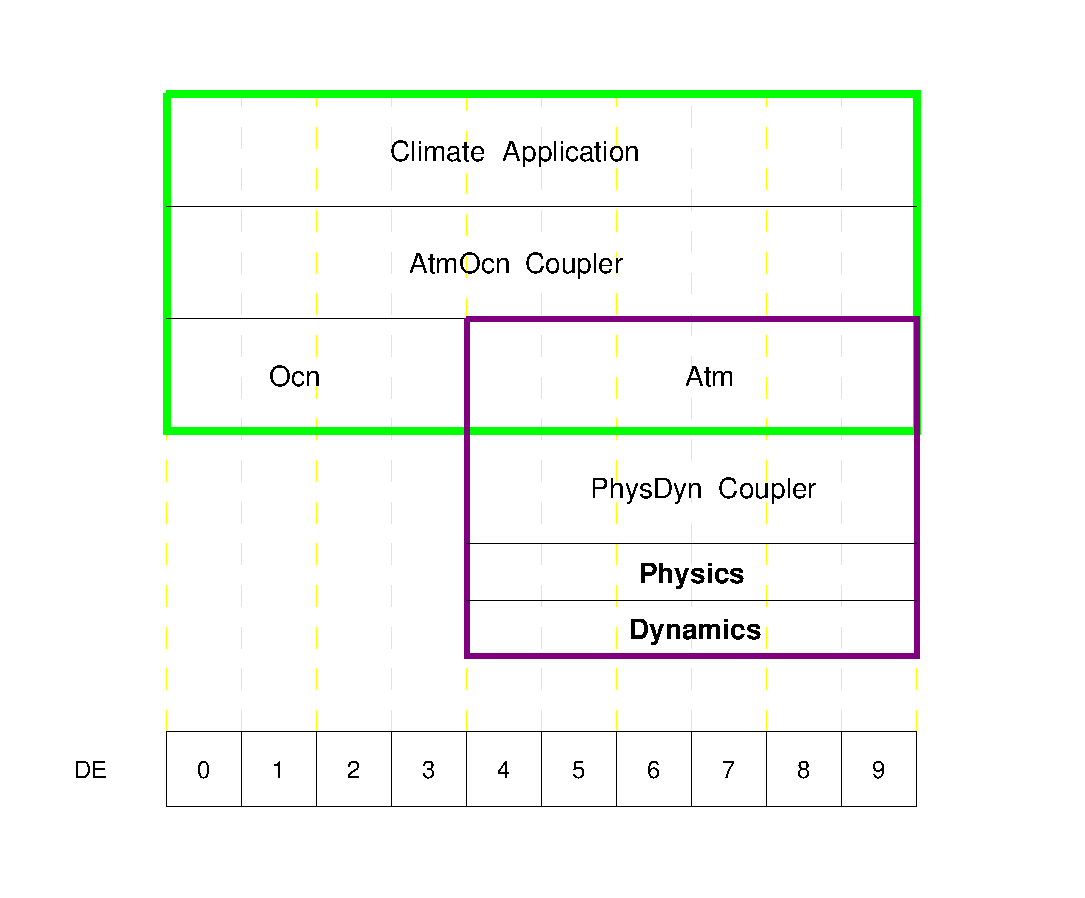
\includegraphics{CouplerScaling.eps}}
\end{figure}


\subsection{Flow of Control}
\label{sec:controlflow}
{\tt Gridded components} have few responsibilities with respect to coupling
to other components.  They do not need to keep track of the data needed
by other components or to provide methods for inter-component 
grid transformations or transfers of data.  They {\it are} responsible for 
providing a description of all of the fields and data they
can export to other components, and for similarly providing a description 
of the data they require in order to run.  These descriptions are
embodied in the {\tt ESMF\_State} class, and the kind of data that they 
represent is identified by the {\tt type} attribute of that class, which can
have an {\tt ESMF\_IMPORT} or {\tt ESMF\_EXPORT} value.  The {\tt State} class
includes metadata information, actual pointers to data 
locations, and default criteria for data validation.  The last of these in its
simplest form may be a bit that is set when data is ready for use.  The ESMF 
will provide methods that enable a user to add or remove fields and data from 
{\tt State}s.  

A {\tt Coupler Component} produces a specification of the sequence of 
operations that are necessary to effect communication between components, 
both scientific and computational, generic and user-defined.  The {\tt Coupler} 
returns these to the {\tt Application} or parent in the form of a set of {\tt Transform} objects 
along with associated sequencing restrictions.  Each {\tt Transform} has a
function pointer to a transform operation and may be bundled with 
associated data, information about coupling frequency, and 
data validation criteria.

The {\tt Application} or parent component initiates the coupling and manages 
its scheduling.  It is responsible for instantiating the {\tt Gridded Component}s
that are exchanging data and instantiating the {\tt Coupler}, for setting up the desired 
sequencing, and making the calls to the methods of the components and 
{\tt Coupler} that effect the exchange.  The parent may partition the 
transforms
for execution among the {\tt Gridded Component}s and the {\tt Coupler}, so that, for 
example, a data send or coupling transformation can occur while a {\tt Gridded 
Component} is executing, without a need for the component to return to the
parent level.  
To disable or rearrange the coupling sequence, a different set of function
pointers can be passed to the component.

The {\tt ESMF\_StateTransform} call executes a {\tt Transform} 
within a {\tt Gridded Component}.  It takes as arguments a
{\tt Transform} object and the component's import or export {\tt State}.  
For {\tt Transform}s that initiate non-blocking sends, a {\tt ESMF\_StateTransformComplete} 
call can check that data  buffers are available for reuse.  This 
call takes the initiated {\tt Transform} object as an argument.

The {\tt ESMF\_StateValidate} call evaluates whether a component's 
import {\tt State} is ready for use.  It may check the entire {\tt State} or 
a specified subset.

Figure \ref{fig:RunApplicationDiagram} outlines the sequence of steps that an ESMF application
executes in a basic simulation scenario. Two gridded components {\it Atmosphere} and {\it Ocean}
are created and two coupler components {\it Atmosphere} to {\it Ocean} and {\it Ocean} to {\it Atmosphere}.
The sequence in figure \ref{fig:RunApplicationDiagram} will be preceeded by the startup procedure illustrated
in figure \ref{fig:ESMFApplicationMain}.

\begin{figure}
\caption[{Basic Run Application}]{Sequence for basic Run Application process.\\}
\label{fig:RunApplicationDiagram}
\scalebox{0.70}{\includegraphics{RunApplicationDiagram.eps}}
\end{figure}

\subsection{Flow of Data}
\label{sec:dataflow}
The design choices we have made enable the user to configure ESMF
applications so that data is transferred from one component to another, 
without requiring that it first be sent via message passing to a
{\tt Coupler} (or even necessarily
copied).  This is likely to be the most efficient way of performing 
inter-component coupling when the components are instantiated on different
{\tt DE} sets.  However, if desired, an application can also be configured so that
data from a source component is sent to a distinct set of {\tt Coupler} 
{\tt DE}s for processing before being sent to its destination.

\subsection{Examples}

Figure~\ref{fig:1waycoupling} shows the sequence of actions involved
in coupling an atmosphere to an ocean.  The vertical axis is time, positive
downward, and the horizontal axis shows the objects that are involved in the
exchange.  Arrow'd lines to text boxes mean that the source of the arrow has 
created the object in the box.  Solid lines to the start of a vertical
box indicate a method call.  Dashed lines indicate a return.  
In this example, the coupling is one-way, so that the ocean 
receives data from the atmosphere but does not send any data back.  Atmosphere
and ocean components are configured for concurrent execution.

\subsubsection{System startup}

The basic startup procedure for an ESMF application is shown in figure \ref{fig:ESMFApplicationMain}. Startup
begins by creating the top-level in figure \ref{fig:couplerscaling}. Any ESMF component could reside at the top-level, so
all ESMF components are created to be consistent with the startup sequence shown in figure \ref{fig:ESMFApplicationMain}.

\begin{figure}
\caption[{ESMF Boot Up Stage}]{The basic startup procedure for
all ESMF applications.}
\label{fig:ESMFApplicationMain}
\scalebox{0.7}{\includegraphics{ESMFApplicationMain.eps}}
\end{figure}

The application begins by creating atmosphere, ocean, and coupler components.
The atmosphere initialization method defines the atmosphere import and export states
(import state creation is not shown) and the ocean initialization method defines
the ocean import and export states (export state creation is not shown).  The
coupler initialization method creates input and output packets, which at this
stage include empty buffers for packing and unpacking data.  The coupler returns a
transform (in this case, perhaps a combined unit change, regrid and communication 
operation) that will occur while the atmosphere 
component is in the midst of its iteration loop.  Some parts of the transform
may be user-defined (i.e., unit changes) and others supplied by the framework
(i.e., regridding and communication).  The application calls the run methods
of the atmosphere and ocean components with the transform provided by the coupler,
which contains different tasks for the two components.  The atmosphere and ocean 
check that their import states are valid as they begin executing concurrently on
different {\tt DE} sets.  At an appropriate time the
ocean component calls a state transform method with its import state and 
the transform it received from the application.  If the frequency criteria
contained within the transform specifies that this is a coupling timestep,
the call 
posts a message passing receive.  When the atmosphere's data is ready to send, 
it calls a state transform method with the transform it was passed and 
its export state.  This call checks the frequency criteria and if it is a 
coupling timestep performs
the unit conversion and regridding, initiates a send
to the ocean and returns.  (Although the calculation is performed on the atmosphere 
{\tt DE}s in this example, the transform could be staged on a separate set of coupler
{\tt DE}s.)  The atmosphere calls a state transform complete call with the transform
as an argument before it proceeds to make any changes to data in the export state
that may still needed.  The atmosphere and ocean proceed to the next 
timestep, and validate their import states as the timestep begins.  

\subsection{Class Descriptions}

The following are brief descriptions of the objects involved in the
ESMF superstructure. The relationship between the key component types (ESMF\_Comp, ESMF\_App, ESMF\_GComp and ESMF\_Cpl)
is shown in the 
class diagram figure \ref{fig:ESMFComponentDiagram}, which shows the position of these component 
types within an application.

\begin{figure}
\caption[{Component Classes}]{The relationship between basic component categories in ESMF.} 
\label{fig:ESMFComponentDiagram}
\scalebox{0.70}{\includegraphics{ESMFComponentDiagram.eps}}
\end{figure}

\subsubsection{Component (ESMF\_Comp)} 
A {\tt Component} is a functionally related computational entity that 
represents a large system.  The {\tt Component} base class defines a set of operations and
attributes common to all {\tt Component}s.  These include methods such as:
initialize, run, finalize, get distribution, get processor list, get status, 
and retrieve information about subcomponents.  
All {\tt Coupler}s, {\tt Gridded Component}s and {\tt Application}s possess 
these methods. 

\subsubsection{Application Component }

The {\tt Application Component} class is responsible for managing those 
functions that relate to an entire scientific application running under ESMF.
The {\tt Application} initialize method 
must be called at the start of any user application operating under the framework, and
the finalize method at its end.  At initialization the {\tt Application} allocates and 
configures any resources needed to run the framework.  The {\tt Application}
class can be queried for information such as an experiment name, model name, and run 
type (ESMF\_INIT, ESMF\_BRANCH, etc.).  

\subsubsection{Coupler Component }
A {\tt Coupler} is a user-customized type of {\tt Component} that 
encompasses all the functionality needed to communicate data between two or 
more {\tt Component}s.  A {\tt Coupler} has a coupling initiation method that 
defines and returns a set of {\tt Transform}s.

\subsubsection{Gridded Component }
\label{sec:griddedcomponent} 
A {\tt Gridded Component} is a user-customized {\tt Component} 
that typically represents a physical system discretized on some spatial grid.
The {\tt Gridded Component} class has methods for writing 
fields and data to an import and export {\tt State}, for verifying that
these states are fully or partially complete, and for returning these
states when queried.

\subsubsection{State (ESMF\_State)}
A {\tt State} is a description of a set of data that a 
{\tt Gridded Component} either needs to run or can make available.  
{\tt State}s
have a {\tt type} attribute that can have values of {\tt ESMF\_IMPORT} or
{\tt ESMF\_EXPORT}.  A {\tt State} may be acted on by a {\tt Transform} object.
As shown in figure \ref{fig:ESMFStateDiagram} and ESMF\_State object contains 
one or more fields or bundles. All components can use states to encapsulate 
data that they export or import. The relationship between states and 
components is shown in figure \ref{fig:ESMFSystemDiagram}.

\begin{figure}
\caption[{ESMF State Contents}]{Contents of an ESMF\_State object}
\label{fig:ESMFStateDiagram}
\scalebox{0.70}{\includegraphics{ESMFStateDiagram.eps}}
\end{figure}

\begin{figure}
\caption[{ESMF State Role}]{ESMF\_State objects are used to transport data
(fields and bundles) between components}
\label{fig:ESMFSystemDiagram}
\scalebox{0.70}{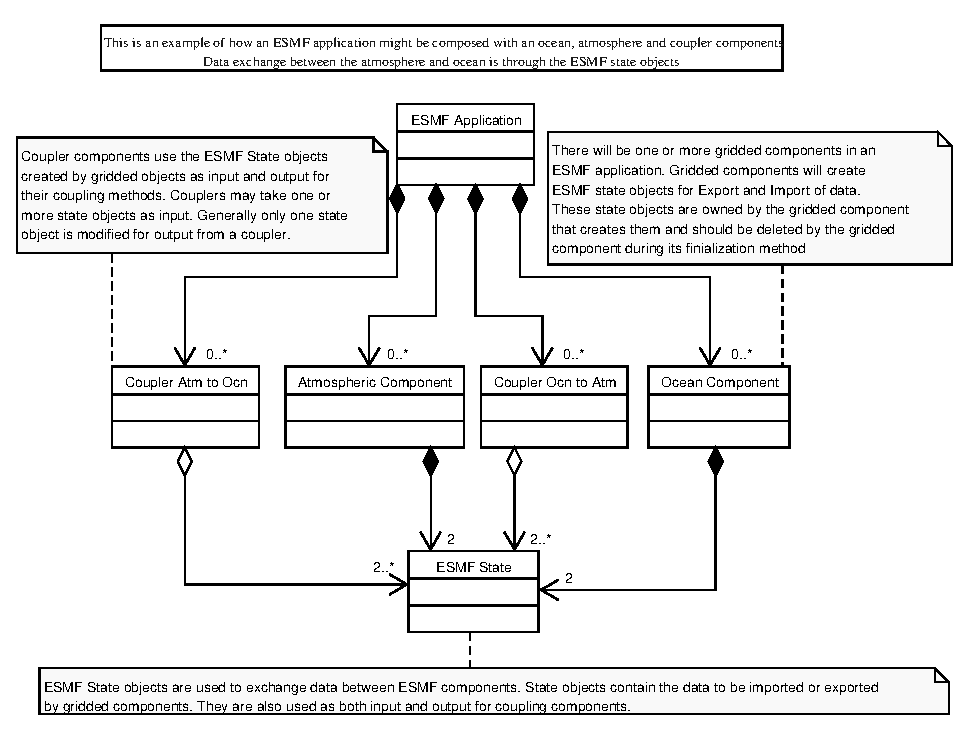
\includegraphics{ESMFSystemdiagram.eps}}
\end{figure}

\subsubsection{Transform (ESMF\_XForm)} 
A {\tt Transform} acts on a {\tt State} or other type of 
ESMF data.  It contains a function pointer to the transformation method
and may contain data necessary to perform the transform, frequency 
criteria and data
validation criteria.  It may relocate data, 
redistribute data, regrid data, change units, any combination of these,
or any other type of operation that the user desires.  









